%!TEX root = ../template.tex
%%%%%%%%%%%%%%%%%%%%%%%%%%%%%%%%%%%%%%%%%%%%%%%%%%%%%%%%%%%%%%%%%%%%
%% chapter3.tex
%% NOVA thesis document file
%%
%% Chapter with a short laext tutorial and examples
%%%%%%%%%%%%%%%%%%%%%%%%%%%%%%%%%%%%%%%%%%%%%%%%%%%%%%%%%%%%%%%%%%%%
\chapter{Proposed Solution}
\label{cha:proposed_solution}
After the problem contextualization, and the description of the related concepts, techniques and studies, this chapter presents the work done so far. Starting with a requirements analysis which includes user interviews and extraction of metrics to conclude in a quantitative way what are the cases where the SQL is used. Continuing with the priority assigned for each problem based on the requirement analysis. A current progress state of the solution developed will be presented, describing the actual development state and a foreseeing schedule of the work plan for the remaining time until the final of the project.

\section{Requirements Analysis}
\label{sec:requirements_analysis}
The project has started with an exploration of the OutSystems Platform data querying tool, the Aggregates, to understand its functionalities and visual approaches used to perform queries visually, as has been described in section \ref{subsec:visual_data_querying}. Meanwhile, not only were identified the expressiveness problems of the visual language, previously mentioned in section \ref{sec:problem_description}, but also usability problems could be perceived in the performance of available actions. 

After that, user interviews have been prepared to explore better the barriers of the tool and understand the impact of the problems in user actions. So, in the interviews, after perceiving the background of the participant, more directed questions were asked to pick up the first responses of the users about the advantages and disadvantages of the visual query tool. This approach promotes that users talk about the more impactful problems for them and the main situations where this tool is useful. Next, it was asked what are the situations when they use SQL to obtain insights about the reason to not use the visual tool to perform these queries. Also, were required that users present examples to explain the problems they have, whenever possible, because this strategy can be useful to understand the impact level of the problem and sometimes show other problems not referred. In addition, when the users did not mention anything about expressiveness problems, direct questions about if they never needed to use these operations in Aggregates were colocated to cover the possibility of forgetting to mention that aspect.

The results reveal that the most novice users, with less than six months of experience, feels that Aggregates are easy to use and covers his necessity, referring also that is easier to learn than SQL. The most experienced users, who use the OutSystems platform to develop applications every day for professional purpose and have a technological background, reported that in the visual tool they cannot have a good understanding of the global view of the query, mainly if many tables, columns and business rules are involved. Switch between tabs in the interface to view the data sources, and the filtering and sorting criteria were other issue presented, as well as the lack of control on the query output \footnote{As referred on section \ref{subsubsec:current_progress}, when a user adds an entity to an Aggregate, all its attributes are added automatically and if the user hides them the output of the query does not change.}. Asked about the aggregation functions, which were implemented when Simple Queries have been replaced by Aggregates, they do not refer any problem with the approach interaction strategy adopted, not considering these new features as a problem that blocks the use of the tool. Furthermore, other usability problems that decrease the users’ satisfaction have been pointed out, like the difficulty to search for a column in the query result, when there are many columns.

The problem analysis was not limited to users interviews, having been complemented with an analysis of the queries executed on the cloud due to perceiving the quantitative representation of the problems detected in the current progress analysis and inspecting the results of the interviews. The queries analysed, which have been extracted in July 2019 from customers’ projects, were built using Advanced Queries \footnote{The option of the OutSystems Platform, invoked on section \ref{subsubsec:previous_work}, that allows the query design in a textual way using a language based on SQL.}.

Firstly, the data set is composed of 214.400 statements, but only 60.8\% were used in this study since only the queries are important for this context and not other instructions like inserts, updates, deletes and transactions. As the last set also has duplicated queries, these were removed and the final queries set used to extract information comprehends 67.828 queries. The operators and clauses were figured out using a SQL Parser developed in JavaScript \footnote{js-sql-parser repository page: \url{https://github.com/JavaScriptor/js-sql-parser}}.

After the abstract syntax trees of the queries were obtained in a JSON file, these were analysed in a program to count the operators and the clauses that are present in the queries. A first analysis can measure the operators that are not supported by the visual tool, since the textual language are the only way to perform these operations. Figure \ref{fig:aggregates_operations_not_supported_stats} summarizes the number of the queries that contain these operations, where the intersection is not null, so there are queries that have two or more of the indicated operations. Thus, each percentage represents the subset of queries that have the operation inside, no matter if they have other operations or not.

\begin{figure}[htbp]
	\centering
	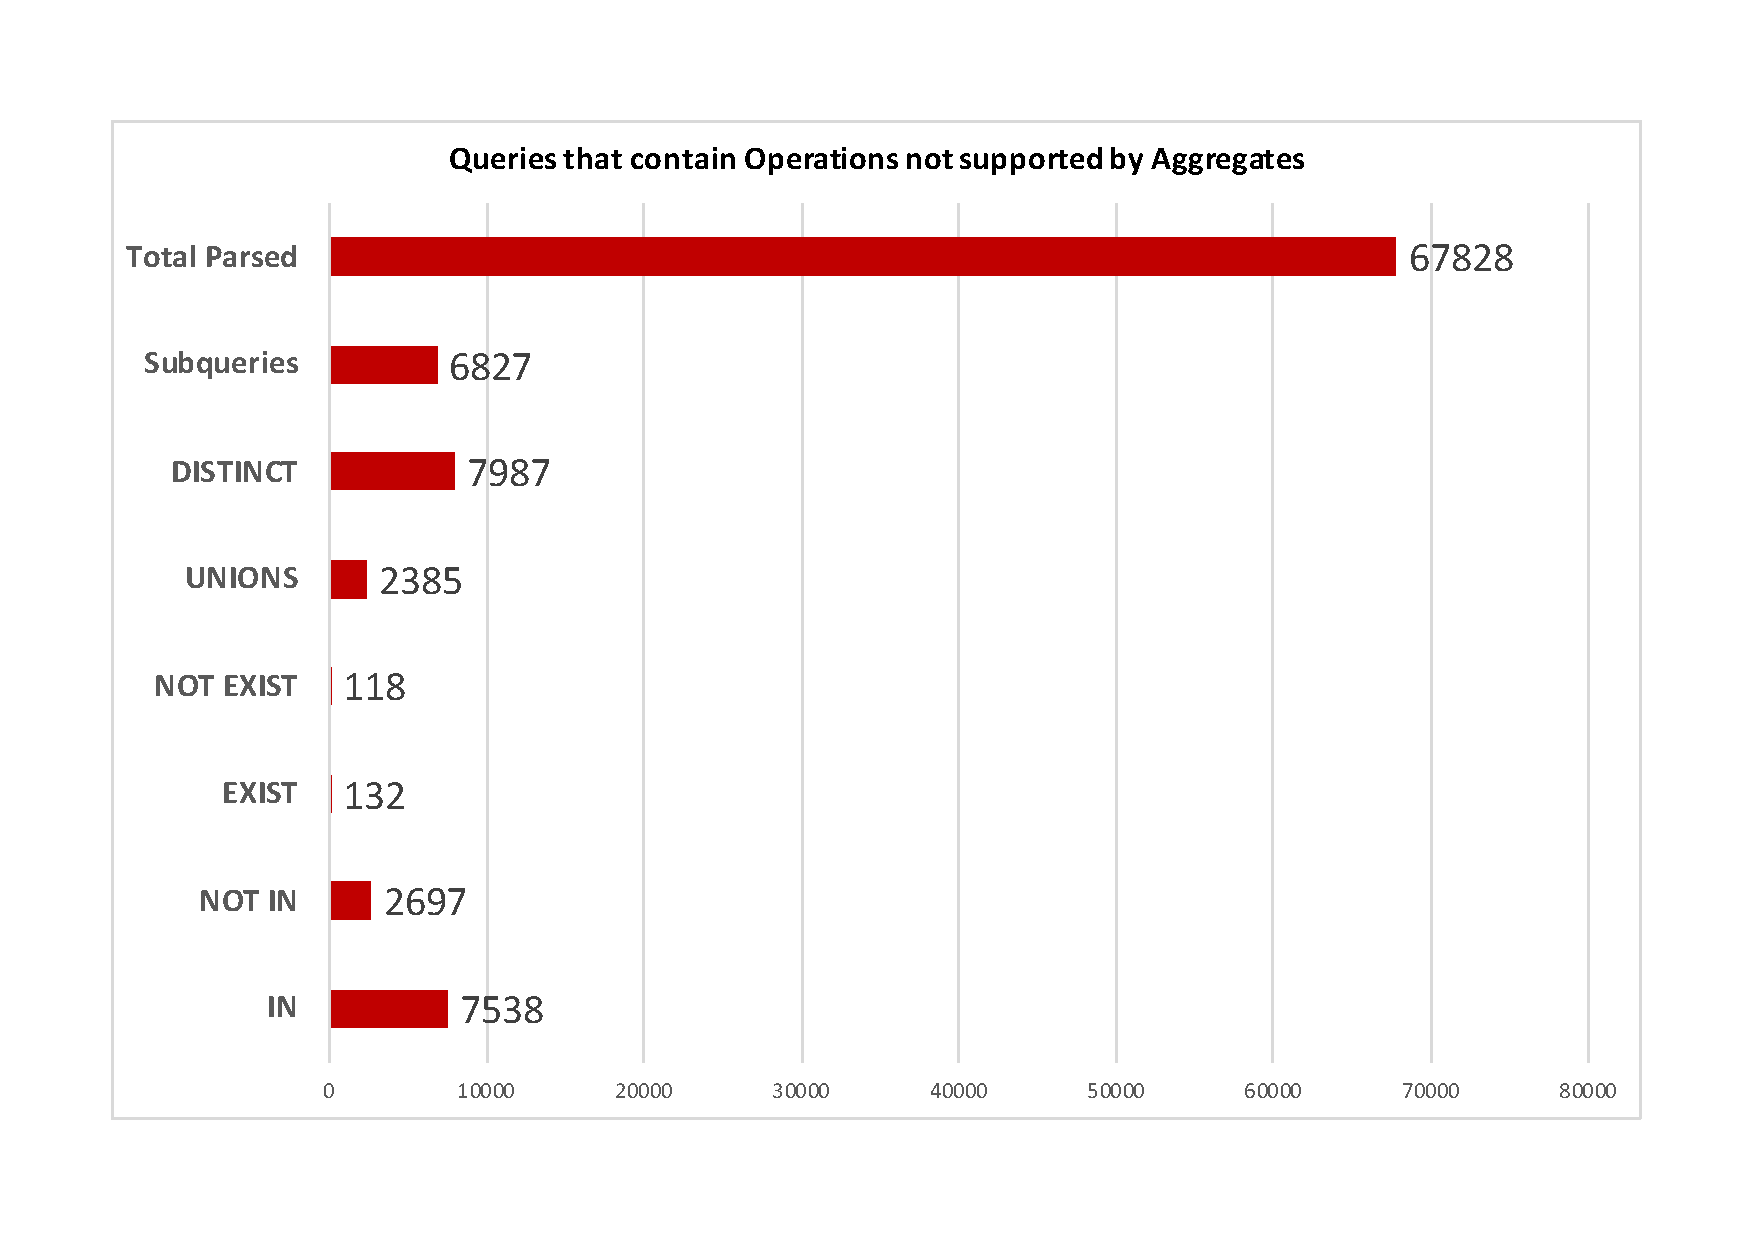
\includegraphics[height=3in]{ChartOperationsNotSupported}
	\caption{Number of the queries that contain operations not supported by Aggregates}
	\label{fig:aggregates_operations_not_supported_stats}
\end{figure}

Furthermore, it was measured how many queries are performed using the textual language but could be designed using Aggregates. Figure \ref{fig:aggregates_supported_vs_not_supported_stats} represents a chart of the results obtained that divide the queries performed in three categories:

\begin{itemize}
    \item Not Supported: Queries which include operations not supported by Aggregates, such as IN, NOT IN, EXIST, NOT EXIST, Unions, Distincts and Subqueries;
    \item Supported by Aggregates: Queries which could be designed totally using Aggregates. These are divided into two subcategories:
    \begin{itemize}
        \item Simpler: Queries which include only operations supported by aggregates excluding the indication of sorting criteria and the use of aggregation functions (e.g. GROUP BY or SUM, AVG, MIN, MAX, COUNT);
        \item More Complex: Queries that are supported by Aggregates excluding the above (simplers).
    \end{itemize}
\end{itemize}

Since user interviews suggested that aggregation functions and sorting criteria were not the main problems. The queries supported by Aggregates were divided to compare the quantitative analysis with the qualitative analysis extracted in interviews. This is important because these operations can be indicated using a different interaction technique where the user changes the query when he is interacting with the query result, as mentioned in section \ref{subsubsec:current_progress}. Thus, this division can be useful to validate the approach used to indicate these aspects of the query.

\begin{figure}[htbp]
	\centering
	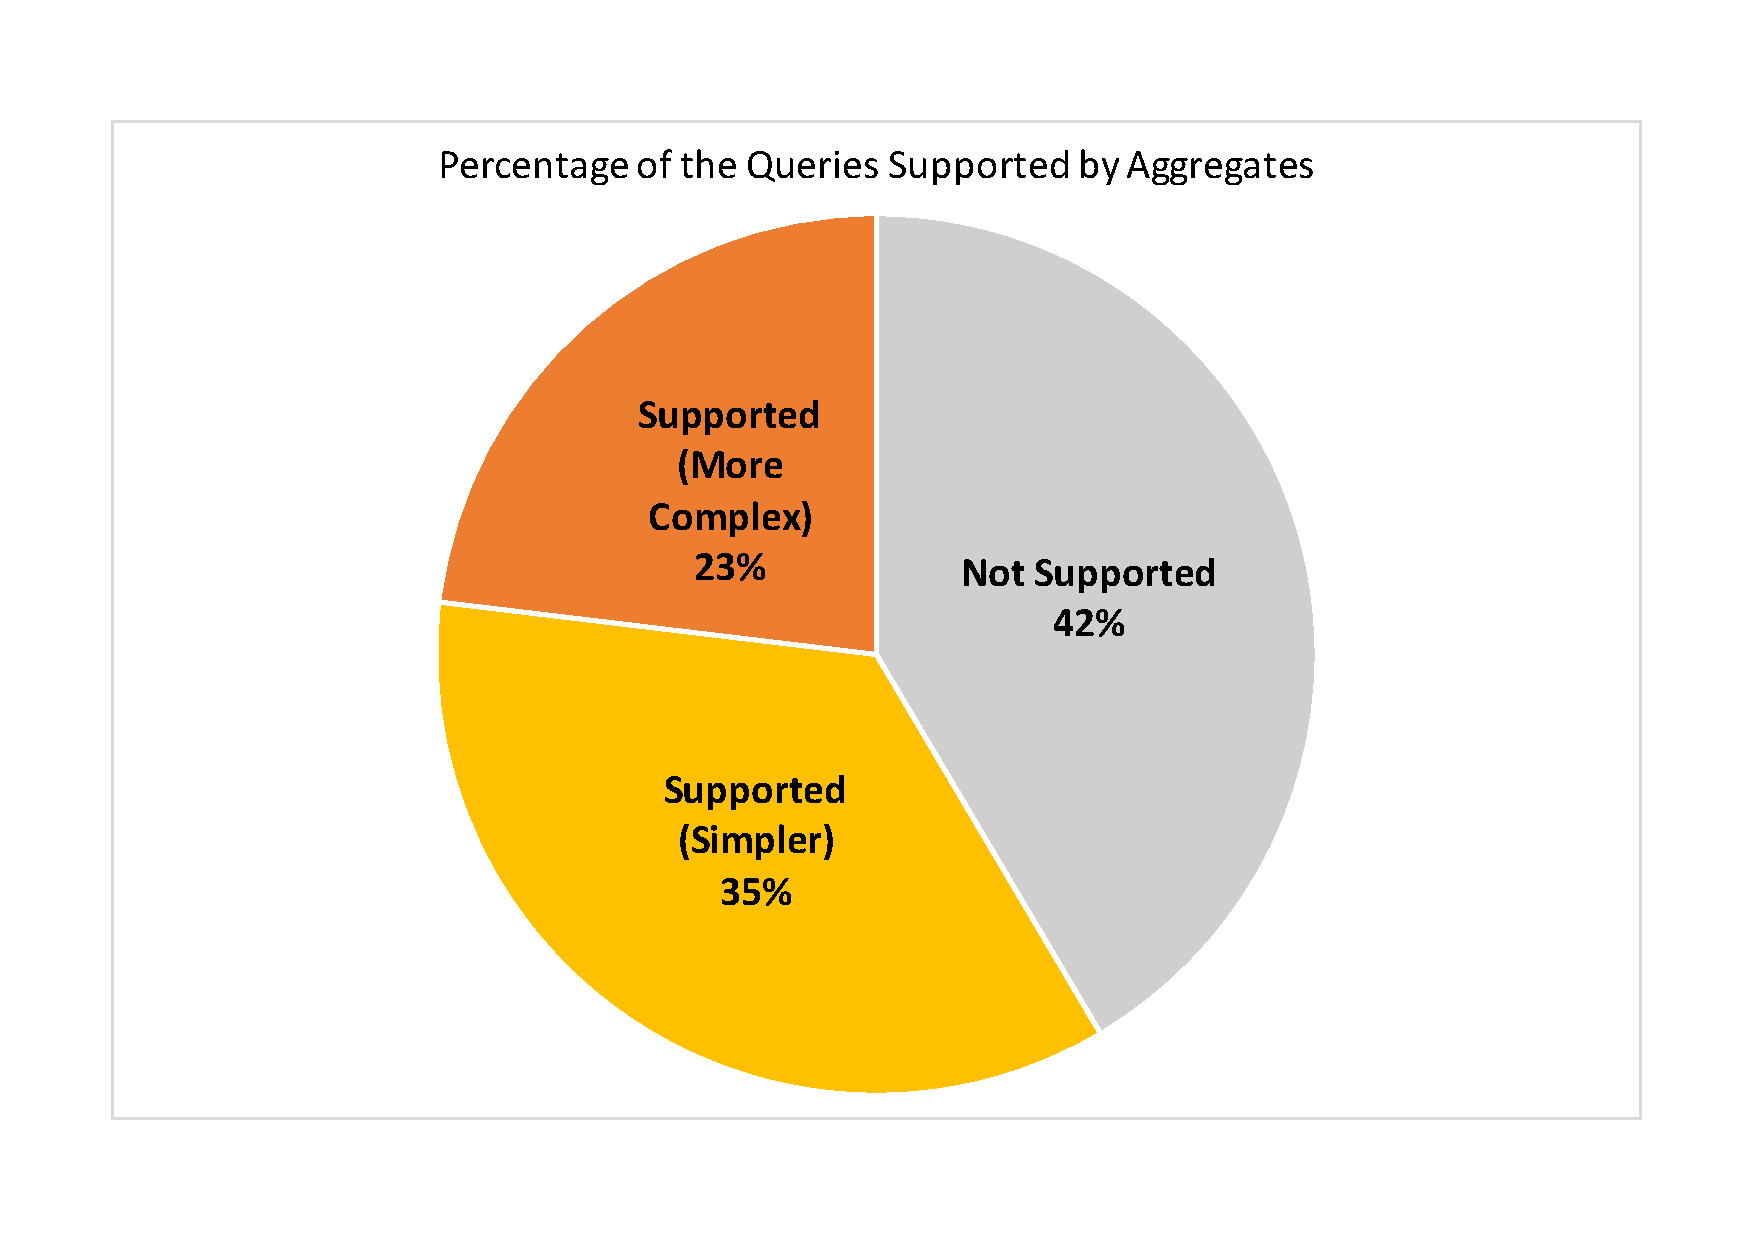
\includegraphics[height=3in]{SupportedVsNotSupportedAggregates}
	\caption{Relationship between the queries that could be designed using Aggregates and the queries which this tool does not support.}
	\label{fig:aggregates_supported_vs_not_supported_stats}
\end{figure}

\section{Scope Definition}
\label{sec:scope_definition}
The results of the quantitative analysis show that there are in conformity with the qualitative analysis results (user interviews). Both of the analysis, leads that the main priority of the project should be the usability improvement of the visual querying tool interface, since not only is the main concerned pointed out by the users, but also has metrics that sustain that hypothesis. In the set of the queries analysed, around 58.5\% could be totally designed using Aggregates, could be an indication that the lack of SQL expression is not the major problem.

Although the results show a small set of queries that are not supported, these expressiveness problems of the visual language can influential the users to change to the textual language, because many users do not like to use different systems to perform identic tasks. So, as the visual language does not support some features users may want to change to the textual language where can perform all the queries.

Under the circumstances, the results were discussed together with the stakeholders to order by priority the problems to be tackled. So, it was decided that the main problem is the usability of the system and regarding the improvement of the visual language expressiveness it was defined that the main priorities are the IN / NOT IN and the DISTINCT operations. Thus, along the project, the main focus will be the improvement of the usability and if is possible to conciliate with the main goal, these two new features of language expressiveness will be studied.

\section{Proposed Implementation}
\label{sec:proposed_implementation}
\textcolor{gray}{Following, will be detailed the intended project, indicating all the problems identified and all the approached that will be adopted.}

\section{Work Plan}
\label{sec:work_plan}

